\chapter{A Compiler for \textsc{x86/32}}

In this section, finally, we will consider a codegenerator for \textsc{x86/32} processor, the principal study
object of the whole course. In this particular chapter we will only deal with the simplest compiler for
straight-line programs, but as the source language evolves the native-code compiler will get more
and more features.

Of course the main question for now is what implementing a native-code compiler amounts to. Luckily, as we will
see shortly, this task is not much different from what we already can do. In order to turn our source program
into machine code we only need to convert it into a text in an \emph{assembly} language. Then we entrust
the \textsc{GCC} toolchain with the task of making the rest of the work~--- compile this assembly program into object file,
link (multiple) compiled object files and some libraries into executable, etc. This approach is by no means
exotic~--- nowdays the majority of compilers are implemented exactly following this roadmap which makes it
possible to reuse all stages of compilation starting from object file generation by many compilers (and thus
avoid of making a lot of similar errors anew).

An important methodological difference of what we are going to do in this chapter is that we \emph{will not}
discuss the operational semantics of the assembly language. The motivation is that this language is very similar
in its generic features to stack machine language, which we already dealt with. As we generate native code from
stack machine, the compiler assumed to be very simple, and its formal description is expected to be superfluous.
On the other hand there are a lot of tiny simple details in machine architecture which would make formal description
boring and cumbersome, so we better discuss them in informal terms. But this does not mean that assembly languages
cannot be properly described in formal terms, and there are lots of witnesses of the opposite.

\section{Hardware Architecture}

In this section we consider some basic principles of digital hardware organization, describe how actual hardware works,
what components it is comprised of, and how it interprets machine program. All these subjects are topics of interest
for the field of \emph{hardware architecture}; we only scratch the surface of this very interesting and important
domain to the minimal extent needed to understand the essence of computations performed by actual hardware.

\begin{figure}[t]
  \centering
  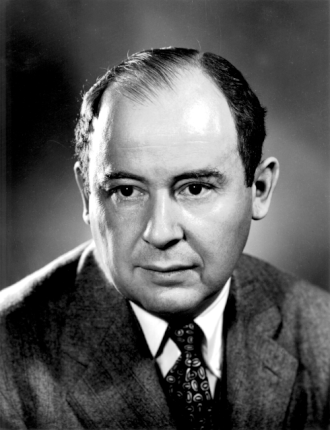
\includegraphics[scale=0.5]{images/JohnvonNeumann.png}
  \caption{John von Neumann}
\end{figure}

From a birds-eye view a hardware computer consists of \emph{memory}, \emph{central processor unit} (CPU), and
\emph{input-output} subsystem. This very general decomposition is called ``von Neumann architecture'' named
after John von Neumann. In von Neumann architecture programs are kept in the same memory as data; this is
sometimes contrasted to so-called \emph{Harvard architecture} where a separate memory is dedicated solely to
keep programs. While the majority of general-purpose computers follow von Neumann architecture the Harvard one can be
found in some embedded devices. The real implementations of both approaches, of course, are much more complicated then
the generic scheme: there can be more than one CPU core, the CPU core itself contains one or more \emph{arithmetic-logic units} (ALU) and
\emph{multiplexers} (MUX) to perform conditional computations, memory subsystem is implemented using \emph{memory controller} and can
incorporate one or more levels of \emph{cache}, there is, as a rule, a separate subsystems to handle software and hardware \emph{interrupts},
support \emph{virtual memory}, \emph{virtualization}, etc. However, the general construct of a \emph{hardwired electronic interpreter}
of programs represented as sequences of bits kept in memory can be easily discovered in all digital programmable devices. This is,
by the way, justifies the central role of the concept of interpreter: there is actually no way to evaluate a program other than
to run it on some (perhaps, hardware) interpreter.

An important observation is that not all details of hardware organization are visible at the application level; some of them are intentionally
designed to be completely transparent to an end-user application. For example, hardware interrupts, virtual memory, cache, etc., as a rule are
invisible for a regular application, which means that a compiler in the \emph{majority of cases} (but not always!) can ignore the presence of
these subsystems. Moreover, a compiler as a rule does not deal with a certain part of hardware functionality and instruction set just
because the source language does not have corresponding abstractions. Finally, as a regular interpreter can be implemented in
various ways even using the same implementation language, hardware platforms also can have different implementations while sharing
the same ``surface'' architecture and instruction set. This surface, or \emph{macroarchitecture} of \textsc{x86/32} is a subject
of our close attention in this chapter. But, first, we consider the very principles digital programmable hardware is based on.

\subsection{Principles of Digital Hardware Organization}

Digital hardware in the vast majority of cases operates on \emph{binary} data. In this form all sorts of data a computer
deals with is represented as sequences of integer numbers in binary representation, i.e. in some variant of positional
encoding radix 2; we assume the reader's familiarity with this construct. The advantage of this representation
is that it only requires from a physical system representing one digit to be in one of two stable states. In real
hardware these two states (0 and 1) are usually represented as different voltage levels measured against some
baseline (ground). Binary representation, however, is not a unique solution from either historical or practical
standpoint: for example, the Babbage's analytical machine (the first known, yet unfinished, project of
a Turing-complete computational device) was designed to operate on decimal numbers, and many modern hardware
digital architectures (including \textsc{x86}) support so-called binary-decimal representation in which
a group of four bits represents (with some redundancy) one decimal digit.

To understand how a hardware can perform computations we first consider a simplest possible arithmetic operation: the
addition of two one-bit numbers $x$ and $y$. As there are only four combinations of all possible values for $x$ and $y$
the result of $x+y$ can be summarized with the following \emph{finite} table:

\[
\begin{array}{cc||c|c}
  x & y & carry\,(x + y) & x\dotplus y \\
  \hline
  0 & 0 & 0 & 0   \\
  0 & 1 & 0 & 1   \\ 
  1 & 0 & 0 & 1   \\
  1 & 1 & 1 & 0 
\end{array}
\]

The somewhat unexpected extra column contains so-called \emph{carry bit}. Indeed, the sum of two one-bit numbers sometimes occupies
more than one bit: 1+1=2(decimal)=10(binary). In general case the result of addition of two $n$-bit numbers can (at most) occupy
$n+1$ bit. When we limit the size of numbers by, say, 32 bits we can eventually arrive at a situation when the result of some
computation can no longer be represented by a 32-bit number. In such case an extra, 33th carry bit can be used to
identify an overflow, a situation when further computations start to deliver unreliable results.

Thus, in a general case the addition of two one-bit numbers delivers \emph{two} bits: the carry one and the partial sum (hence the
denotation ``$\dotplus$'').
If we look closely at the table above we can discover that the carry bit is the conjunction of the operands and the partial
sum is exclusive or:

\[
\begin{array}{rcl}
  carry\,(x + y) & = & x\wedge y\\
  \phantom{(}x\dotplus y\phantom{)} & = & x\oplus y
\end{array}
\]

This constitutes an important observation: we will be able to perform arithmetic computations in hardware as long as we manage to implement
boolean operators. There is a whole theory of \emph{boolean circuits} which studies the theoretical properties of computations
performed by the networks of interconnected primitive boolean connectives.

Let us assume that we, indeed, can implement boolean operations using some primitive hardware units (\emph{gates}); depict those as
shown in Fig.~\ref{gates}. Each gate has two \emph{inputs} (wires on the left side) and one \emph{output} (a wire on the right side). 
Then the following interconnection of gates constitutes a one-bit \emph{adder}:
 
\begin{figure}[t]
  \begin{subfigure}[t]{0.3\textwidth}
    \centering
    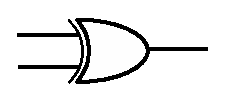
\includegraphics[scale=0.6]{images/06-01.eps}
    \caption{``xor''}
    \label{gates-xor}
  \end{subfigure}
  \begin{subfigure}[t]{0.3\textwidth}
    \centering
    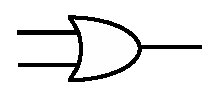
\includegraphics[scale=0.6]{images/06-02.eps}
    \caption{``and''}
    \label{gates-and}
  \end{subfigure}
  \begin{subfigure}[t]{0.3\textwidth}
    \centering
    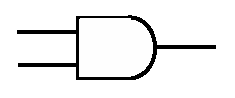
\includegraphics[scale=0.6]{images/06-03.eps}
    \caption{``or''}
    \label{gates-or}
  \end{subfigure}
  \caption{Logical gates}
  \label{gates}
\end{figure}


\begin{figure}[h]
  \centering
  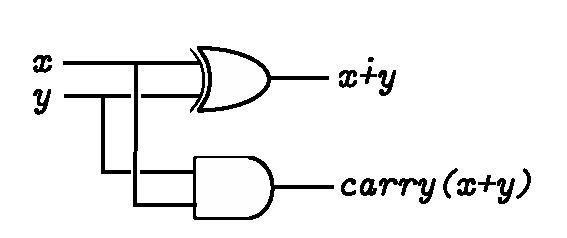
\includegraphics[scale=0.6]{images/06-04.eps}  
\end{figure}

Indeed, this simple circuit literally encodes the table for ont-bit addition.

Imagine now that we want to add two \emph{two-bit} numbers $x_1x_0$ and $y_1y_0$. By the very nature of
binary positional encoding these two-bits numbers represent natural numbers $2\times x_1+x_0$ and
$2\times y_1+y_0$. Let us calculate their sum:

\[
2\times x_1 + x_0 + 2\times y_1+y_0 = 2\times (x_1+y_1) + (x_0+y_0)
\]

But, again, we have to make sure that all coefficients of the degrees of 2 are either 0 or 1; in the
expression above this requirement can be violated (take $x_0=y_0=1$). To fix this remember that we
can express the results of one-bit additions $x_1+y_1$ and $x_0+y_0$ in terms of partial sums and carry bits.
The easiest way to sort things out is to determine which coefficients of degrees of 2 these bits
contribute to:

\begin{itemize}
\item $x_0\dotplus y_0$ contributes to the coefficient of $2^0$;
\item $carry\,(x_0+y_0)$ contributes to the coefficient of $2^1$;
\item $x_1\dotplus y_1$ also contributes to the coefficient of $2^1$;
\item $carry\,(x_1+ y_1)$ contributes to the coefficient of $2^2$;
\end{itemize}

Thus, $x_0\dotplus y_0$ gives us the least significant bit of the overall sum. As both $carry\,(x_0+y_0)$ and 
$x_1\dotplus y_1$ contribute to the same coefficient, we have to add them as well, obtaining yet another
partial sum and carry bits. The partial sum

\[
(carry\,(x_0+y_0))\dotplus(x_1\dotplus y_1)
\]

now is the only bit contributing to the coefficient of $2^1$ (i.e. second-to-the least significant bit of the
overall sum). However, the carry bit

\[
carry\,(carry\,(x_0+y_0), x_1\dotplus y_1)
\]

now contributes to the coefficient of $2^2$ and has to be added to $carry\,(x_1+ y_1)$, which would potentially
give us another two bits. Fortunately, it can be easily observed that

\[
carry\,(carry\,(x_0+y_0), x_1\dotplus y_1)
\]

and

\[
carry\,(x_1+y_1)
\]

can never be equal 1 at the same time. Indeed, let $carry\,(x_1+y_1)=1$. But then $x_1\dotplus y_1=0$, and
$carry\,(carry\,(x_0+y_0), x_1\dotplus y_1)=0$. Thus, their sum is just a disjunction.

These observations can be summarized with the following boolean circuit for \emph{two-bits adder}:

\begin{figure}[h]
  \centering
  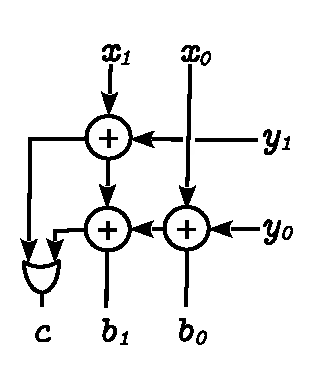
\includegraphics[scale=0.7]{images/06-05.eps}
\end{figure}

Here encircled nodes abbreviate one-bit adders with horizontal output edges associated with carry bits and
vertical ones~--- with partial sum bits. With proper efforts (and enough time) these nodes can be substituted
by the actual circuits for one-bit adders which would give a complete decomposition for two-bit adder in terms of
primitive gates.

Use similar ideas we can scale up the expressive power of boolean circuits almost infinitely. Combining two-bit adders
gives us three-bit adders, etc. Being capable of adding numbers we can multiply (as multiplication of
finite numbers can be expressed in terms of finite number of additions); using the representation in binary complement
form we can use complement and addition for subtraction, which allows us to express division and taking a reminder, etc.
Finally, we can easily express conditional calculations in binary logic: let us have a one-bit condition (``true'' or ``false'') $c$ and
two $n$-bit numbers $x=x_{n-1}\dots x_0$ and $y=y_{n-1}\dots y_0$. Then

\[
(x_{n-1}\wedge c)\dots(x_0\wedge c) \vee (y_{n-1}\wedge \neg c)\dots(y_0\wedge \neg c) 
\]

corresponds to a conditional construct

\begin{lstlisting}[mathescape=true]
    if $c$ then $x$ else $y$ fi
\end{lstlisting}

Generalizing this construct we can implement a choice of one of $2^n$ values depending on $n$-bit condition, which
gives us an implementation of memory. Thus, with just a few types of logical gates we can implement an impressive
variety of computations.

But how the gates themselves are implemented? In the evolution of hardware multiple ways were explored and utilized
starting from purely mechanical appliances made of gears, springs, shafts, etc., through simple electrical
devices with relays and vaccuum tubes to the nowdays semiconductor technologies. We consider a very simple implementation
of logical gates using \emph{relays} since it does not require any specific knowledge of electronics.

\begin{figure}[t]
  \begin{subfigure}[t]{0.5\textwidth}
    \centering
    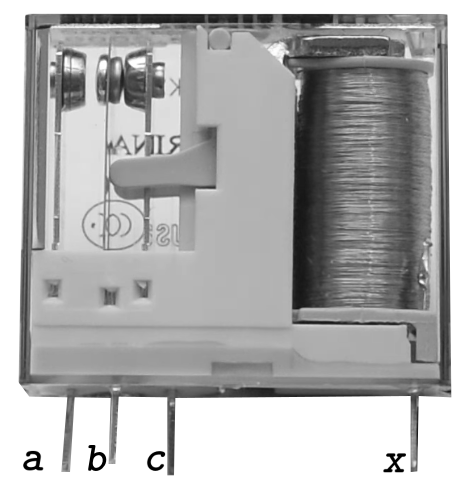
\includegraphics[scale=0.3]{images/06-07.png}
    \caption{Idle state}
    \label{relay-default}
  \end{subfigure}
  \begin{subfigure}[t]{0.5\textwidth}
    \centering
    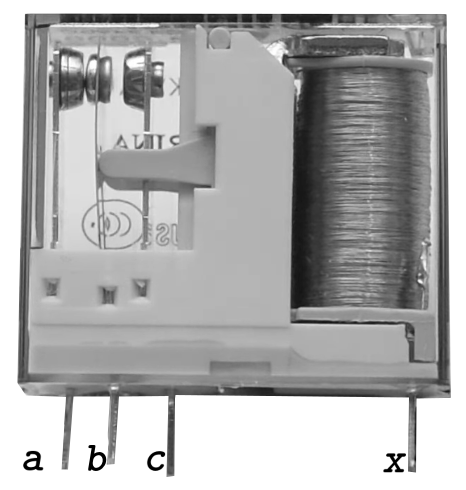
\includegraphics[scale=0.3]{images/06-06.png}
    \caption{Powered state}
    \label{relay-powered}
  \end{subfigure}
  \caption{A relay}
  \label{relay-example}
\end{figure}

A relay is a simple electro-mechanical device which typically consists of a \emph{solenoid} (an electrical wire coiled over
a cylindrical conductor core) and a group of controlled electrical contacts, one of which is mechanically connected to the solenoid's core.
A relay has a few inputs/outputs:

\begin{itemize}
\item control input wires which are directly connected to the solenoid;
\item controlled inputs/outputs wires which are connected to the contacts the relay controls.
\end{itemize}

A relay usually operates in two states. In the idle state when no electrical current flows the solenoid the contact group commutes
controlled wires in some default manner. But when electric power is applied to the solenoind it produces magnetic field which
makes the core to reswitch the contacts and change the way the controlled contacts commute.

As an example consider a simple relay in Fig.~\ref{relay-example}. Here the contact $x$ is control one, $a$, $b$ and $c$~--- controlled.
In the default state (Fig.~\ref{relay-default}) when no power is given to $x$ the contacts $b$ and $c$ are commuted, $b$ and $a$ are not.
However, when an electric power is applied to $x$ (Fig.~\ref{relay-powered}) the commuting scheme between $a$, $b$, and $c$ is
changed: now $a$ and $b$ are commuted, $b$ and $c$ are not.

\begin{figure}[t]
  \centering
  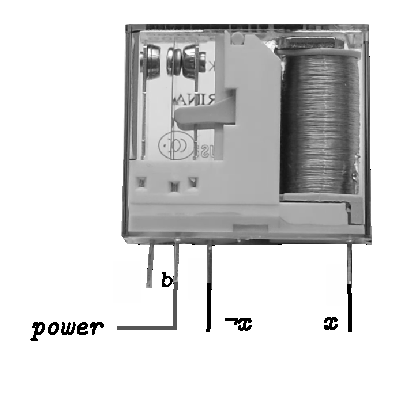
\includegraphics{images/06-08.eps}
  \caption{Relay-based negation implementation}
  \label{relay-negation}
\end{figure}

The simplest gate we can implement with the relay is negation (Fig.~\ref{relay-negation}). Here we left pin $a$ unconnected, $b$ is
constantly connected to the power source. Now, in the idle state when no signal is given to the pin $x$ there is a signal on the
pin $c$. When a signal is given to the pin $x$ the relay recommutes the controlled pins, and the signal on $c$ disappears. Thus,
$c$ holds a signal when $x$ does not and visa versa.

To implement, say, a conjunction we need \emph{two} relays as there are two input arguments which require two input
pins (one of each relay). We can successively connect power source and pins $a$ and $b$ of each relay as it is
shown in Fig.~\ref{relay-conjunction}. Now, in order to have a signal on the pin $b_1$ we need two signals on
pins $x_0$ and $x_1$ simultaneously, which means that $b_1=x_0\wedge x_1$. 

\begin{figure}[t]
  \centering
  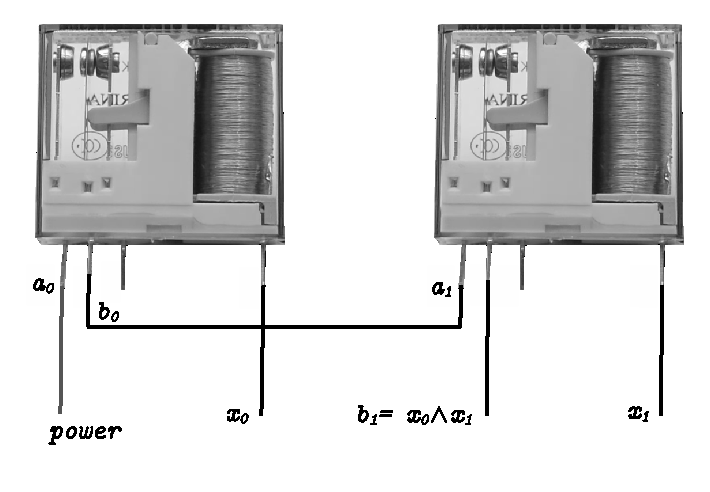
\includegraphics{images/06-09.eps}
  \caption{Relay-based conjunction implementation}
  \label{relay-conjunction}
\end{figure}

It is well-known that conjunction and negation form a complete set of boolean connectives: any other can be expressed
using these two. For example,

\[
\begin{array}{rcl}
  x\vee y & = & \neg (\neg x \wedge \neg y) \\
  x\oplus y & = & (x \vee y) \wedge \neg (x \wedge y)
\end{array}
\]

etc. Thus, we already can have a relay-based implementation (albeit not very efficient and reliable) for all imaginable
hardware.

In practice nowadays the majority of hardware devices is manufactured in the form of \emph{integrated circuits}: meshes
of millions of primitive devices printed (or, more specifically, \emph{etched}) on a common semiconductor substrate (\emph{wafer}).
As a rule multiple individual integrated circuits are placed on a single wafer, which is later cut into smaller
pieces~--- \emph{dies}. Each die occupies just a few square millimiters of area, but using a microscope its
layout can be visually observed and even photographed, resulting in a \emph{die shot} (see Fig.~\ref{die-shot}).
Finally, each die is packed into a protective plastic or ceramic case with a number of electrical pins sticking out, which
finally constitutes a microchip. We do not present any picture of a microchip here since if you never saw one you
probably have chosen a wrong course to study\footnote{As of 2023.}.

\begin{figure}[t]
  \centering
  \includegraphics[scale=0.07]{images/Intel_Pentium_II_Dixon_die_shot.jpg}
  \caption{Intel Pentium III Die Shot}
  \label{die-shot}
\end{figure}

Althought technologically the whole process is drastically different from manual combining of relays, ideologically
it is very similar and each primitive semiconductor device (such as transistor) logically functions pretty much
like a relay. 

\subsection{Synchronous Design}

Now we know how to implement a computation in hardware: we can construct a circuit of gates which,
given a certain set of binary signals on its inputs, will provide an expected result in the form of binary signals on
its outputs. There is, however, a number of important observations:

\begin{itemize}
\item A hardware is rarely (if ever) designed to perform just a single computation. As a rule
  we expect it to work for a large amount of inputs which means that these inputs are going to
  change over time.
\item All hardware gates have some \emph{latency}~--- correct output signals do not appear immediately, they
  take some time to establish. Moreover, this time can be different for different output signals since
  the length of a \emph{datapath} from inputs to a concrete output can be different. Moreover, this
  time can depend on the concrete state of inputs due to conditional computations.
\item Since digital signal is just a voltage level when it changes (say, from 0 encoded as 0V to 1 encoded as +3V) it, actually,
  takes all intermediate voltage levels from 0V to +3V.  
\end{itemize}

Thus, when we change the signals on inputs the output values start \emph{incoherently} change over time. In some time
the correct output values are established, but this very moment we can change the inputs, again, destructing this correct
output value. Thus, when the input changes unpredictably the output values also oscillate unpredictably, making it
impossible to filter out correct states from intermediate ones.

One way to cope with this problem is \emph{synchronuous design}. In synchronuously designed hardware the whole
mesh of gates is divided into synchronized blocks. Within these blocks the signals are propagated asynchronuously, i.e.
as we already described. However, on the inputs and outputs of these blocks the signals are \emph{latched}
using certain type of gates and a dedicated periodical signal called \emph{clock}. This signal is generated by devices
similar to those used in conventional quartz wristwatches; its distinctive feature is square-shaped waveform with
a constant period. In Fig.~\ref{clock-diagram} an example of clock signal diagram is shown. The clock signal changes
its value from 0 to 1 and back over and over again with a given period. The change of the clock signal from 0 to 1 (or visa versa)
is used to toggle the latches to re-lock their values (indicated on the figure by white triangles). Thus, input and outputs
signals of asynchronuous blocks remain constant during the period which eliminates their oscillation. The clock period is carefully
chosen in such a way that each asynchronuous block have enough time to stabilize its correct outputs by the end of the period
regardless the contents of its input signals. 

\begin{figure}[t]
  \centering
  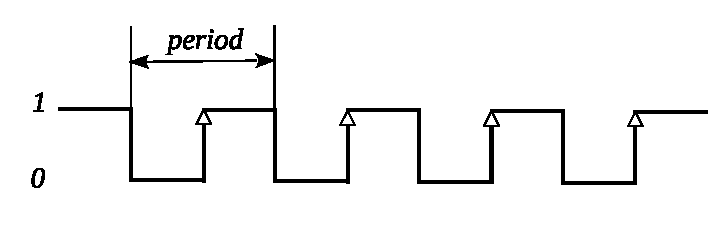
\includegraphics[scale=0.7]{images/06-10.eps}
  \caption{Clock Diagram}
  \label{clock-diagram}
\end{figure}

From this we can derive a number of important observations:

\begin{itemize}
\item Synchronuous hardware logically operates in a discrete time: it consumes inputs discretely (once per a clock period) and
  outputs results discretely (once per a clock period).
\item This time discretization is global (the same for the whole device)\footnote{There actually can be designs in which different
subparts of a device function with different clock rates, but the implementation requires special efforts.}.
\item The period is determined by an asynchronuous block with the highest latency. Thus, contrary to a conventional beleif, in hardware
there is spoiling a wedding for one that is missing.
\end{itemize}

Besides synchronuous design there is also a symmetrical idea of \emph{asynchronuous} hardware organization according to which
different computational units individually agree with each other on the reliability of their results. This idea has its
merits and drawbacks; however, the vast majority of hardware devices nowdays is synchronuos, so we stick with this model for
the time being.

\subsection{Programmability, Instruction Cycle, and Pipelining}

The idea of a \emph{programmable} device originates from a very natural observations. The first, and the most important, is
that with a programmable device it is possible to perform almost any kind of computations by fitting in an appropriate program.
But even if we are interested in performing only a limited set of computation the programmability allows us to improve
both \emph{resourse usage} and \emph{throughput}.

To illustrate the idea consider a simple expression graph shown in Fig.~\ref{expression-example}. Imagine that we 
need to calculate only this expression but for many consecutive inputs. We can, of course, implement a monolitic
boolean circuit to evaluate this particular expression. However, in this case, first, the circuit would contain
duplicate parts: two identical adders and two identical multipliers.
Second, the longest datapath would consist of one adder and two multipliers (there is also a path with two adders and
one multiplier, but the latency of a multiplier is larger than that for an adder),
which means   that in synchronuous design the period of the clock has to be large enough to let one addition and two multiplication to
provide reliable results. If $L_a$ is the latency of the adder and $L_m$ is the latency of the multiplier then the period of
clock signal has to be larger than $L_a + 2\times L_m$ (assuming that the whole circuit is implemented asynchronuosly).

In programmable case we can build a circuit with just one adder and one multiplier and some extra logic to
change the interconnection between them. This interconnection in controlled by a \emph{machine program} which is
generally is kept in memory. To make the things work we also need some extra memory cells (denote them \verb|r0|, \verb|r1|, etc.),
called \emph{registers}, which reside inside the cirsuit itself and, unlike general-purpose memory, can be accessed
almost immediately. A machine program is an array of \emph{instructions}, each of which 



\begin{figure}[t]
  \centering
  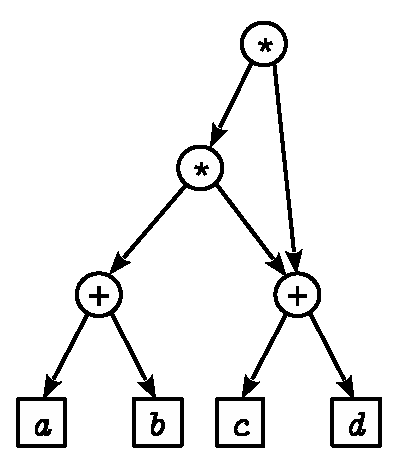
\includegraphics[scale=0.7]{images/06-11.eps}
  \caption{An Example of Expression Graph}
  \label{expression-example}
\end{figure}

\subsection{x86 Macroarchitecture}

\section{Code Generation with Symbolic Interpreter}

\section{}


